\subsection{How much of the gain comes from modeling clutter?}
A high output sensing ratio in a clutter-free simulation and a high ratio in a cluttered environment answer different design questions. We separate them with paired interventions on the transmit kernel, receive kernel, and evaluation environment. Each of 12 new seeds (47001--47012) supplies a channel draw for each user count $K\in\{4,8\}$, reused across SINR requirements of 0, 8 and 16 dB. The 72 cases use the same 32 tones, 100 W budget, target coefficient, and underlying clutter environment as the MATLAB benchmark. We use the Python six-allocation fixed-proposal solver throughout this ablation. Each physical return is audited against the original user constraints and total power. The ideal kernel is available for evaluation.

Let $0$ denote the zero cold-clutter map, $\widehat{\mathcal C}$ the estimated map, and $\mathcal C$ the ideal scoring map. In the \emph{joint-aware} design, both transmit and receive updates use $\widehat{\mathcal C}$. In the \emph{blind} design both use $0$, and the returned beams are scored under $\mathcal C$. A third design retains the blind transmit beams and updates only the receiver by \eqref{eq:mvdr} under $\widehat{\mathcal C}$. All three experience the same true clutter and the same $R_{\eta,n}$. Two physical controls change the environment: first we evaluate the blind transceiver with cold scattering absent and $R_{\eta,n}$ retained; then we redesign and evaluate with only spatially white receiver noise, $R_{\eta,n}=\sigma_r^2 I$, using the tutorial's per-tone thermal-noise variance $\sigma_r^2$. The last condition measures a sensing SNR. The target coefficient remains fixed under the benchmark normalization in \eqref{eq:radar}.

\begin{figure*}[t]\centering
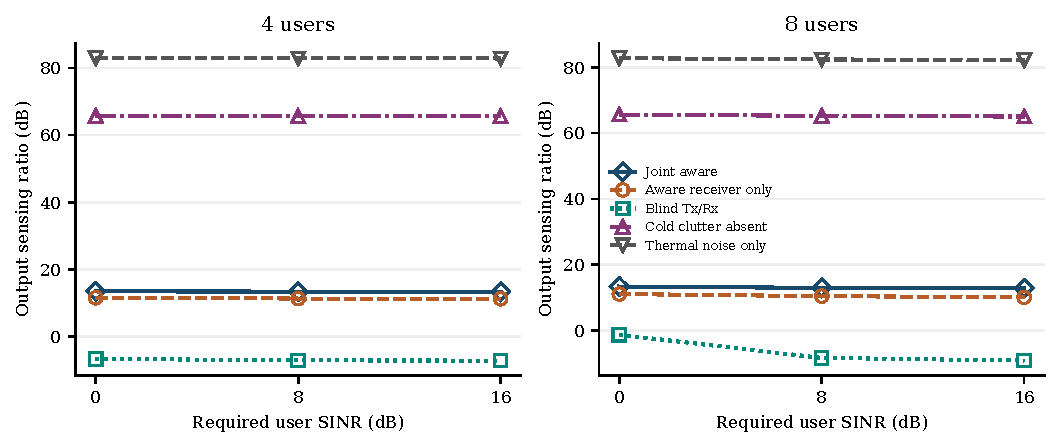
\includegraphics[width=.88\textwidth]{clutter-ablation.pdf}
\caption{Physical clutter removal and clutter-blind design. Each point is the median output sensing ratio over 12 matched channel seeds. The three lower curves share the same physical scattering and additive disturbance. The two upper curves change the physical disturbance. The thermal-only curve retains receiver noise.}\label{fig:cold}
\end{figure*}
At four users and 8 dB, the median true SCNR was $-7.01$ dB with a blind transceiver, 11.37 dB after adapting only its receiver, and 13.44 dB with joint design (Fig.~\ref{fig:cold}). At that operating point, removing cold clutter physically yielded 65.70 dB; thermal noise alone yielded 82.84 dB. For a fixed blind pair, removing cold clutter must increase the score by exactly $10\log_{10}(1+D_c/D_a)$, where $D_c$ and $D_a$ are respectively the cold and additive terms in the denominator of \eqref{eq:ratio}. This identity was checked on every pair. The large absolute levels arise under the tutorial's fixed-power normalization and disturbance scales.

Across all 72 pairs the median gain of joint awareness over blind design was 20.77 dB (95\% seed-cluster bootstrap interval 9.01--21.91 dB). Against the same blind transmitter with an adapted receiver the gain was 2.19 dB (1.99--2.33 dB). The latter comparison isolates the incremental value of redesigning the transmitter when the receiver already has the estimated clutter model. The intervals resample 12 seed clusters, preserving the six operating conditions within each cluster, using 4000 bootstrap resamples. They quantify channel variation within this environment.

\subsection{Conventional transmit directions and communication feasibility}
To isolate the transmit design, maximum-ratio transmission (MRT), zero forcing (ZF) and regularized ZF (RZF) all receive estimated-kernel MVDR filtering. Comparisons of conventional precoders also appear in Wang \emph{et al.}~\cite{wangclutter}; the following power rules target our multitone per-user constraints. Using the normalized channel matrix $G_n$ defined earlier, the direction matrices before column normalization are $G_n$ for MRT and $G_n(G_n^{\mathsf H}G_n+\delta I)^{-1}$ for ZF ($\delta=0$) and RZF ($\delta=0.1$). This fixed regularizer defines the RZF control.

For direction $v_{nk}$ assigned to user $k$, set $b_{ki}=|h_{nk}^{\mathsf H}v_{ni}|^2$ on tone $n$. Define $F_{ki}=\gamma'_{nk}b_{ki}/b_{kk}$ for $i\ne k$, $F_{kk}=0$, and $d_k'=\gamma'_{nk}\sigma_c^2/b_{kk}$. If the spectral radius of $F$ is below one, the minimum user powers are $(I-F)^{-1}d'$, obtained by saturating the QoS inequalities. The inverse is the nonnegative series $\sum_{j\ge0}F^j$, establishing componentwise minimality. If the spectral radius reaches one, a nonnegative left Perron eigenvector applied to $p\ge Fp+d'$ rules out feasibility since $d'>0$. Any surplus system power is distributed equally over tones on their normalized target-steering projections into the user null space. An unavailable fixed-direction design counts as a feasibility failure; its SCNR is omitted.
\begin{figure*}[t]\centering
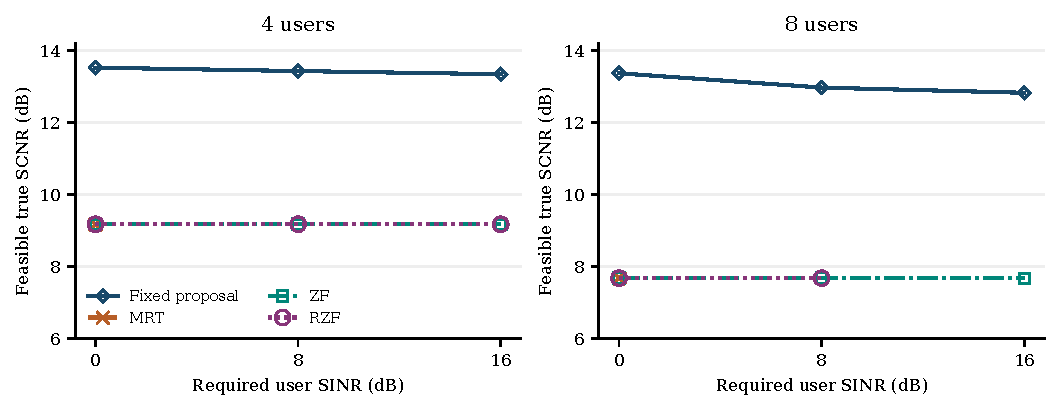
\includegraphics[width=.87\textwidth]{precoder-comparison.pdf}
\caption{True SCNR under identical physical clutter. Each visible point uses all 12 draws for that setting. MRT has feasible points only at 0 dB. RZF is infeasible for all draws at eight users and 16 dB. Similar values among feasible conventional methods reflect their shared null-space sensing beam and power rule.}\label{fig:precoders}
\end{figure*}
Joint design and ZF each returned 72 feasible designs. RZF returned 60 and MRT returned 24. Against ZF, the paired median gain was 4.69 dB (4.63--4.75 dB). Against RZF and MRT, the paired medians were 4.59 and 4.93 dB on their respective feasible subsets. Different subsets prevent interpreting those two medians as a ranking of the conventional methods. The 20.77-dB clutter-awareness result and the 4.69-dB ZF comparison use different controls; neither measures a gain from learning.
\begin{figure*}[t]\centering
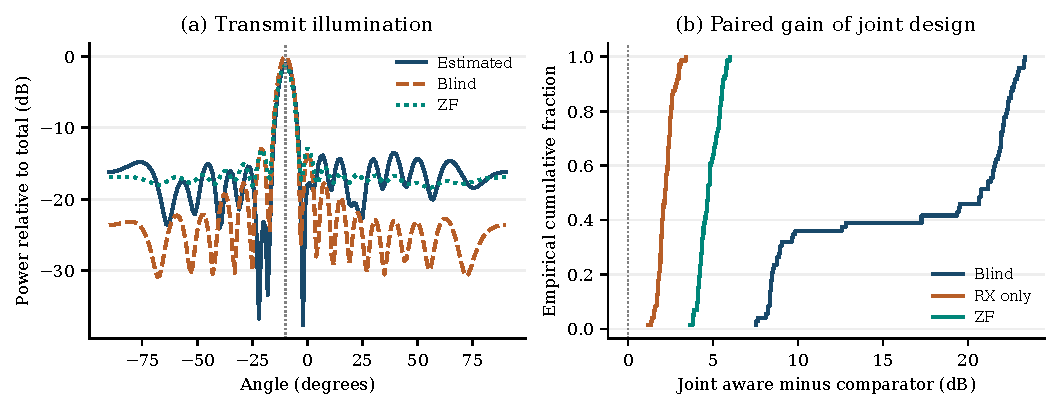
\includegraphics[width=.87\textwidth]{physical-mechanism.pdf}
\caption{(a) Transmit beampattern at four users and 8-dB required SINR, averaged in linear units over 12 channels. At angle $\theta$ we plot $10\log_{10}[\sum_n a_{N_t}(\theta,n)^{\mathsf H}Q_na_{N_t}(\theta,n)/P]$ after averaging; the common reference preserves differences in target illumination. The vertical line marks the target at $-10^\circ$. (b) Empirical distribution of paired true-SCNR gains over all 72 cases. Receive processing and the clutter kernel also determine output SCNR.}\label{fig:pattern}
\end{figure*}
